\documentclass[tikz,crop,border=0pt]{standalone}
\usepackage{pgfplots}

\begin{document}
\pgfplotsset{width=10cm,height=8cm,compat=1.13}
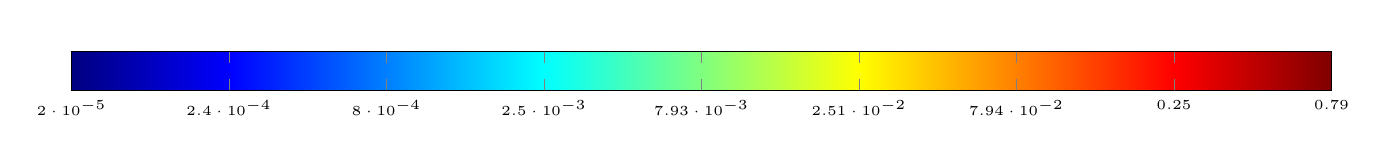
\begin{tikzpicture}
\begin{axis}[
    hide axis,
    scale only axis,
    height=0pt,
    width=0pt,
    colormap/jet,
    colorbar horizontal,
    point meta min=-4.1,
    point meta max=-0.1,
    colorbar style={
        width=16cm,
        xtick={-4.1,-3.6,...,-0.1},
        xticklabel=\pgfmathparse{10^\tick}\pgfmathprintnumber\pgfmathresult,
        xticklabel style={font=\tiny}
    },
]
    \addplot [draw=none] coordinates {(0,0)};
\end{axis}
\end{tikzpicture}

\end{document}
